The ${H_{\infty}}$ control technique is an optimization-based approach composed of two main stages. In the first one, it is formulated a minimization norm problem of the closed-loop system between specific signals. Then, in the second stage, the optimization problem based on the \textit{generalized plant} is solved.
\newline
The aim is to design a \textit{K} to attenuate the influence of $w$ on the signals $z$ in the closed-loop system. In particular, the \textit{generalized plant} has two inputs, $w$ and $u$, and two outputs, $z$ and $y$:
\begin{itemize}
	\item \boldmath$w$ represents the exogenous input. In this case, it is composed of several signals: the position reference and the state and measurement noises. Regards the torque disturbances discussed in \cref{sec:FD_control}, these are not considered because they become relevant only when the masses are rotating at constant speed. Indeed, in the position control this behavior is neglected since the masses are stopped after the transient.
	\item \boldmath$u$ is the control input.
	\item \boldmath$z$ is the regulated output, which is required to be kept \textit{small}. This signal is made by the output of the shaping functions, that will described later on.
	\item \boldmath$y$ is the measured output.
\end{itemize}

\section{\onedof\ system}
The system is made by 4 states and 2 sensors, that are a potentiometer and an encoder. Their noises are respectively indicated by vectors $n_x$ of dimension 4 and $n_y$ of dimension 2. Thus, $w$ will be of dimension 7:

\begin{equation}
	w=
	\begin{bmatrix}
		\theta_{1_{ref}} & n_x & n_y
	\end{bmatrix}^{T}
\end{equation}

Considering the state and measurement noises written above, it is needed to specify their variances. The state one ($\tilde{Q}$) is obtained through an empirical tuning, as discussed in \cref{sec:Kalman_filter}, while the sensors one ($\tilde{R}$) is computed with methods discussed in \cref{sec:sensors}.

The \textit{generalized plant} $P(s)$ is:
\begin{equation}
	P(s)
	=
	\left[
	\begin{array}{c|cc}
		A & B_{w} & B \\
		\hline
		C & D_{w} & D	
	\end{array}
	\right]
\label{P(s)}
\end{equation}

where $A$,$B$,$C$ and $D$ are the system matrices, while $B_{\dot{x}\omega}$ and $D_{y\omega}$ are:

\begin{equation}
	B_{w}=
	\begin{bmatrix}
		zeros(n_x,1) & \sqrt{\tilde{Q}} & zeros (n_x,n_y)
	\end{bmatrix}
\end{equation}

\begin{equation}
	D_{w}=
	\begin{bmatrix}
		zeros(n_y,1) & zeros (n_y,n_x) & \sqrt{\tilde{R}}
	\end{bmatrix}
\end{equation}

The shaping functions illustrated in \ref{Weighting functions scheme1dof} are used to weight the different signals in different control frequency bandwidth. 
For what concerns $W_e$, it is preferable to weight more the error at low frequencies to reduce as much as possible its value at steady state. Whereas for $W_u$, the goal is to limit the bandwidth of the control action, with a focus on low frequencies, to avoid the amplifier to  work at its extreme performance. This choice leads to a less aggressive regulator and so it is expected to have some oscillations that the control action is not able to compensate. In order to reduce this behavior, an additional shaping function which limits $\theta_{1}$ at high frequencies is designed.

\begin{figure*}[h]
	\centering
	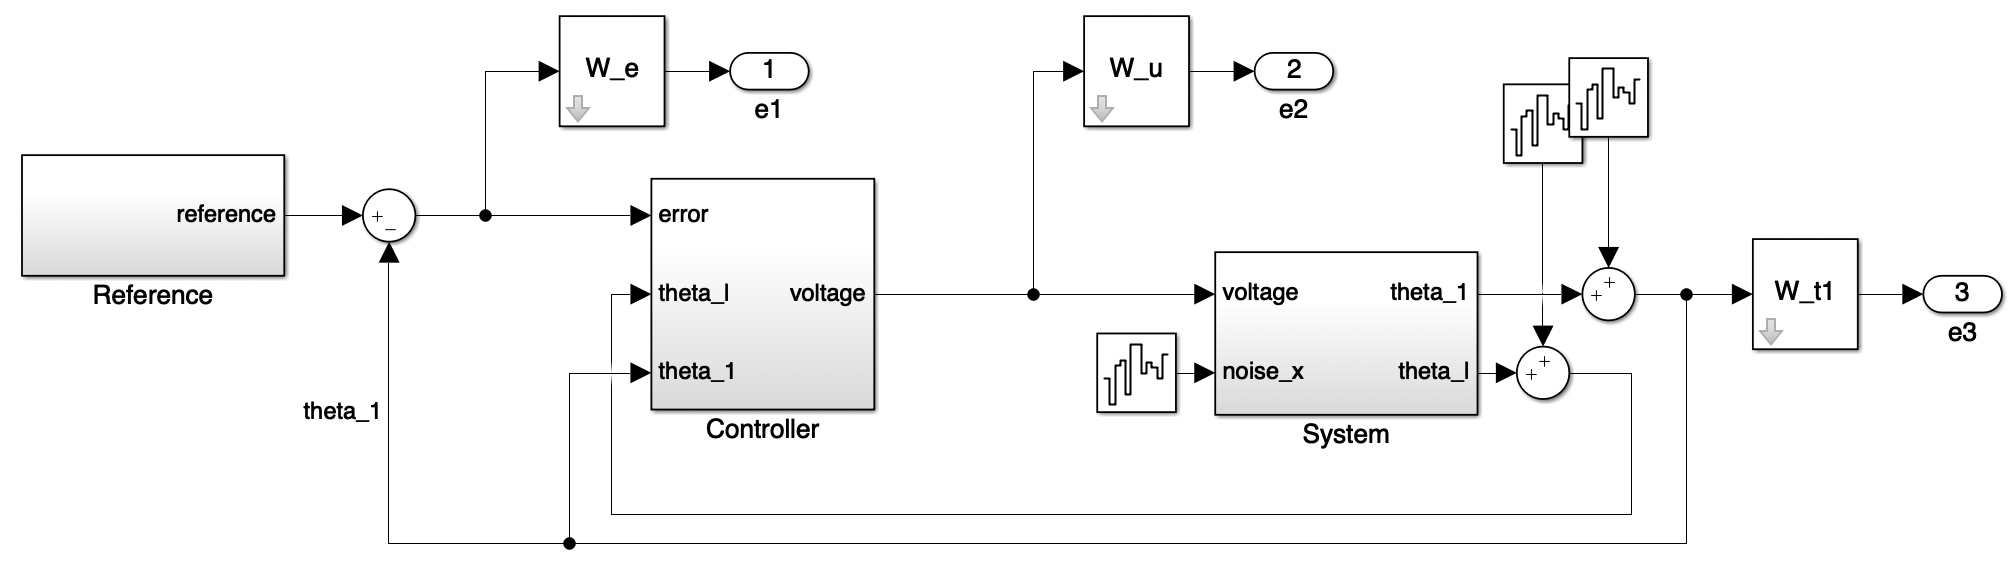
\includegraphics[scale=0.3]{Wfig1dof}
	\caption{Weighting functions scheme}
	\label{Weighting functions scheme1dof}
\end{figure*}
Starting from this reasoning, the weighting function have been empirically tuned in the laboratory. The final choices are:

\begin{equation}
	W_e=
	\frac{s+30}{s+0.01}
	\\
	,
	\\
	W_u=
	\frac{s+0.1}{s+150}
	\\
	,
	\\
	W_{\theta_{1}}=
	\frac{s+10}{0.01s+2}
\end{equation}

\begin{figure*}[h]
	\centering
	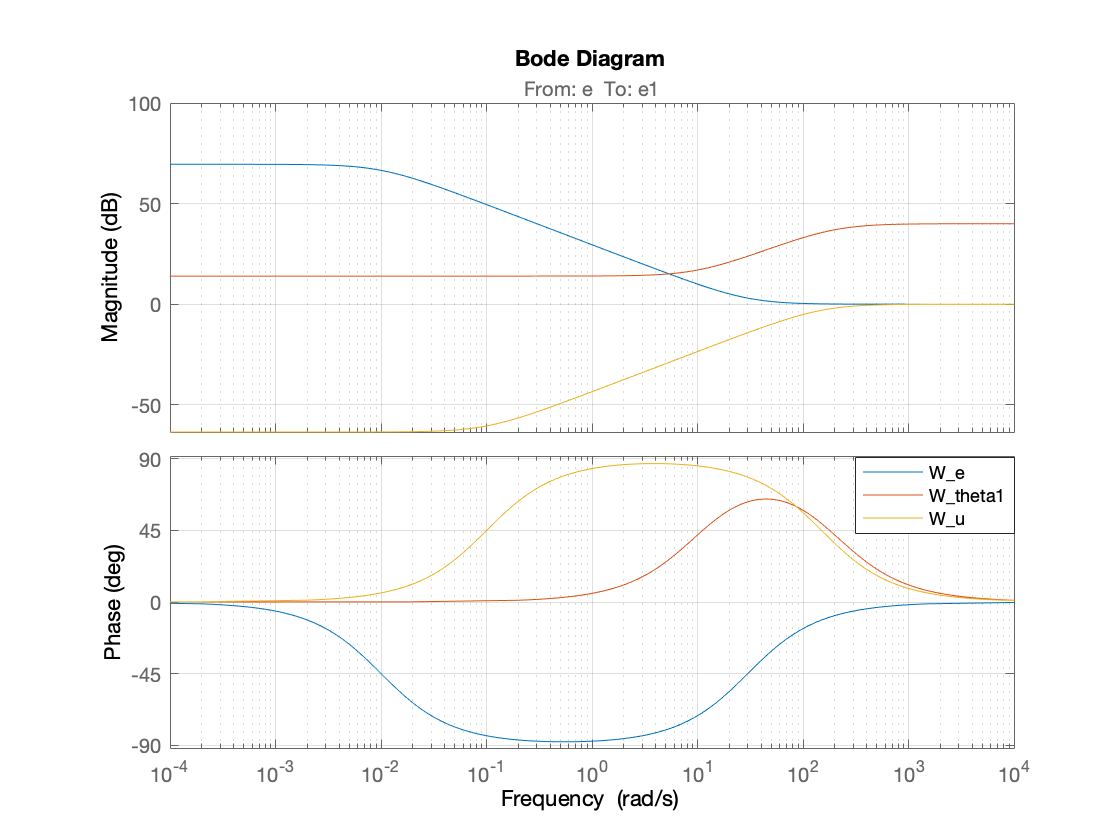
\includegraphics[scale=0.3]{W1dof}
	\caption{Weighting functions}
\end{figure*}

 In \cref{fig:posH1dof}, it is observable how the simulation and the laboratory data share the same settling time, despite the fact that the $\gamma$ obtained by the $H_\infty$ is $6.34$ and thus the solution can't be considered acceptable. Anyway, this one is the fastest ever obtained throughout the project work. Furthermore, in both the experiments it was able to reach the reference at steady state.
 
 \begin{figure*}[h]
 	\centering
 	\begin{subfigure}{0.5\columnwidth}
 		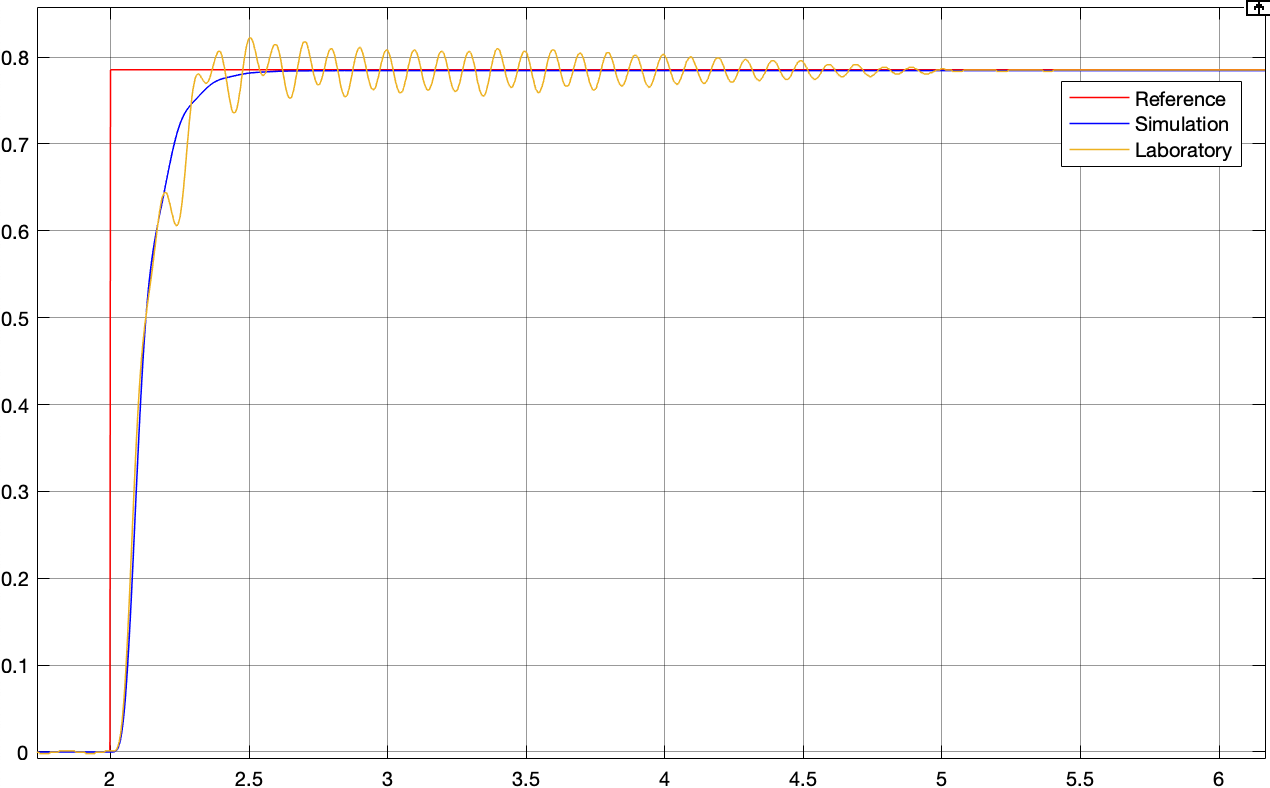
\includegraphics[scale= 0.37]{posH1dof}
 		\caption{Position}
 	\end{subfigure}
 	\begin{subfigure}{0.45\columnwidth}
 		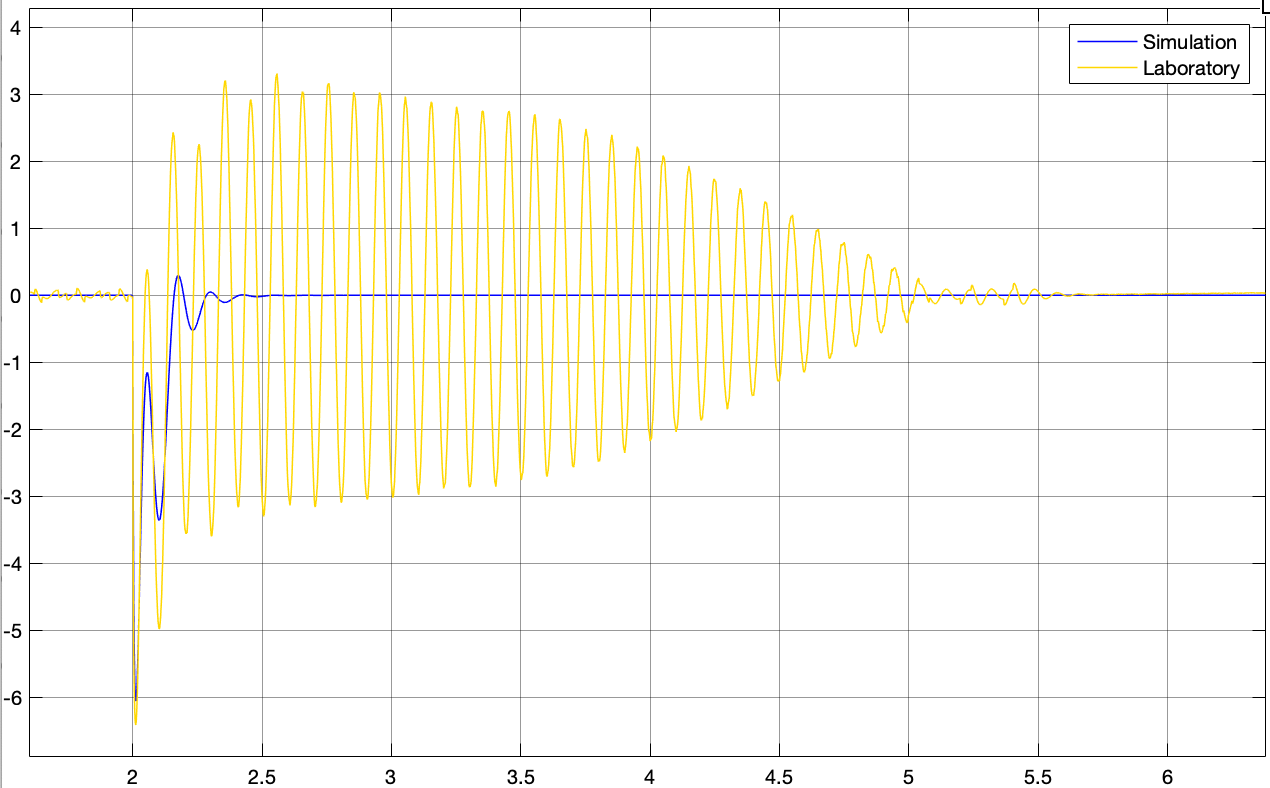
\includegraphics[scale=0.37]{voltH1dof}
 		\caption{Voltage}
 	\end{subfigure}
 	\caption{Position step response}
 	\label{fig:posH1dof}
 \end{figure*}

Due to a lack of time, the final result is not satisfactory, tuning all the parameters of a $H_\infty$ problem is a hard work that requires a lot of time due to the high number of degrees of freedom. 
\newpage
\section{\twodof\ system}
In this scenario, the states are 6 and the sensors are 3, for this reason $w$ is composed of 10 signals:

\begin{equation}
	w =
	\begin{bmatrix}
		\theta_{2_{ref}} & n_x & n_y
	\end{bmatrix}^T
\end{equation}
Coherently with the \onedof~case, the variances matrices are built keeping the same values as in the Kalman filter formulation:

The definition of the \textit{generalized plant} $P(s)$ is the same explained starting from \cref{P(s)}. Then, the following weighting functions are implemented:

\begin{figure*}[h]
	\centering
	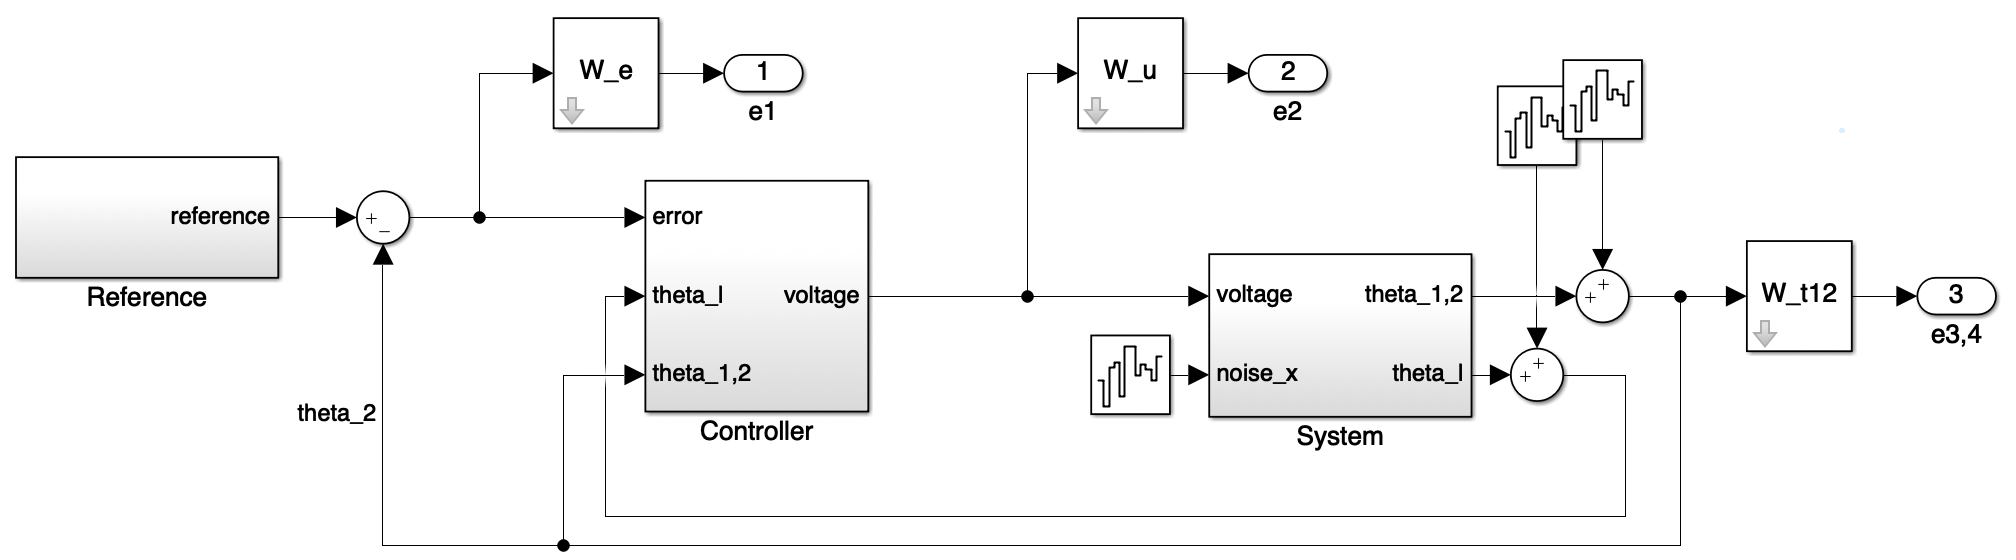
\includegraphics[scale=0.3]{Wfig2dof}
	\caption{Weighting functions scheme}
	\label{Weighting functions scheme2dof}
\end{figure*}

The reasoning followed to design these functions are the same written above and the differences between them are due to a different tuning made at the laboratory. To overcome as possible the oscillation issue, we penalize homogeneously the whole control frequency range. In a first moment, just one weighting function $W_{\theta_{2}}$ on the second mass has been considered, but in this way the first mass was too much oscillatory. Another shaping function to penalize the high frequencies of the first mass position has been tuned.

\begin{equation}
	W_e=
	\frac{s+30}{2s+0.02}
	\\
	,
	\\
	W_u=0.9
	\\
	,
	\\
	W_{\theta_{1}}=
	\frac{s+10}{0.01s+2}
	\\
	W_{\theta_{2}}=
	\frac{s+10}{0.01s+2}
\end{equation}

\begin{figure*}[h]
	\centering
	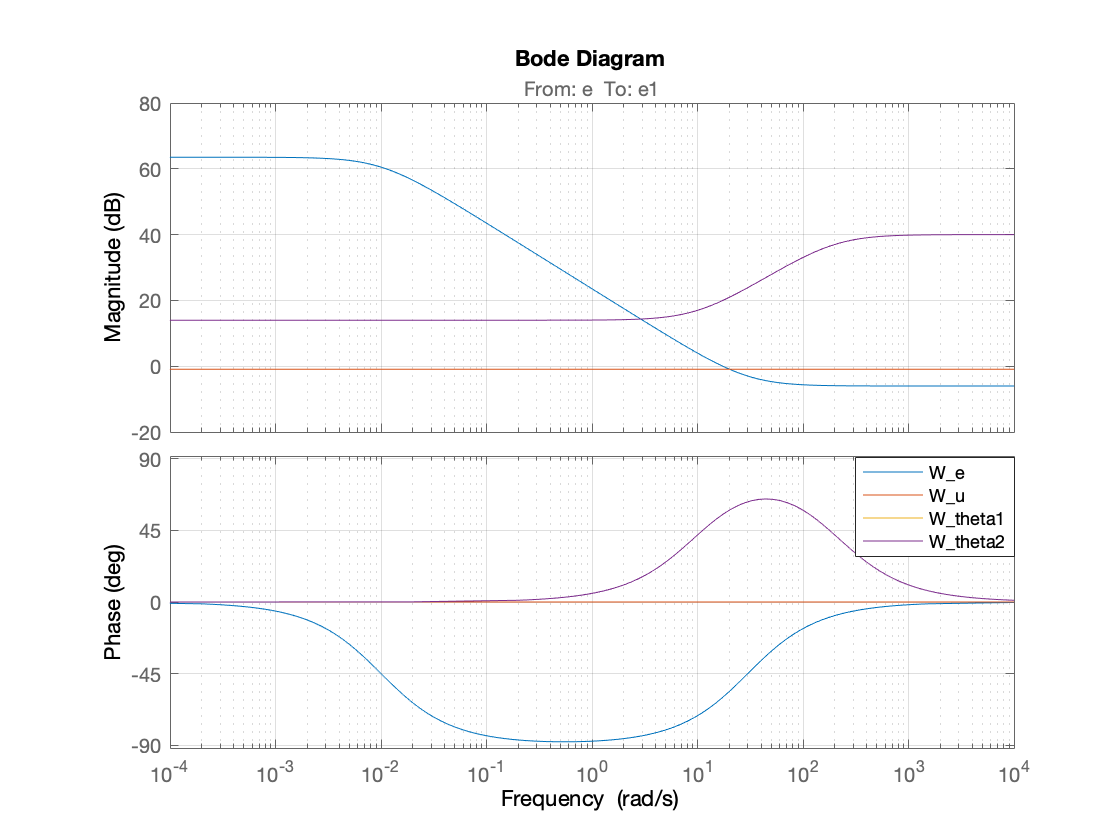
\includegraphics[scale=0.3]{W2dof}
	\caption{Weighting functions}
\end{figure*}


From the plots in figure \ref{fig:posH2dof}, a significant improvement with respect to the solution of the \onedof\ scenario can be noticed. Although there are a few oscillations, this result could be considered acceptable. Unfortunately, the $\gamma$ of the $H_\infty$ problem is 7.43, this means that the weights still are not tuned very well. Most likely there exist better solutions, but due to lack of time we did not manage to explore them.

 \begin{figure*}[h]
	\centering
	\begin{subfigure}{0.5\columnwidth}
		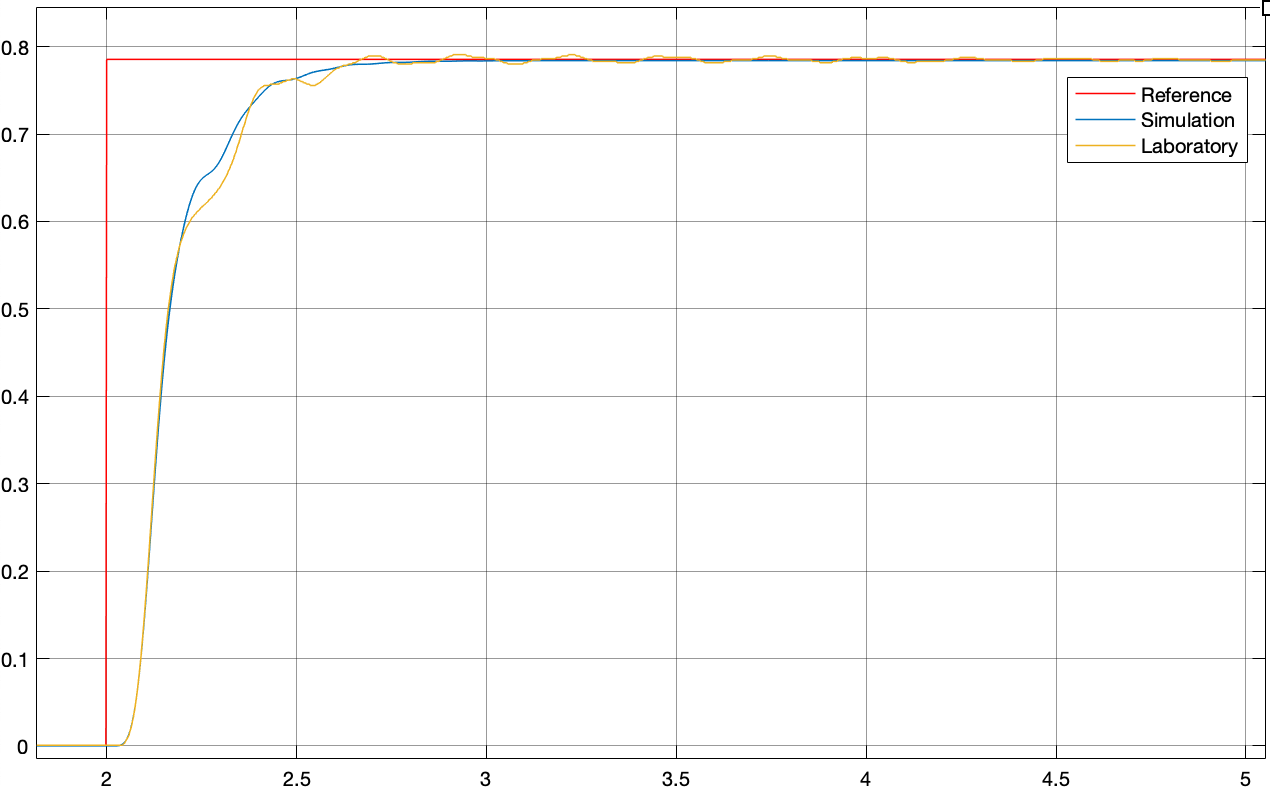
\includegraphics[scale= 0.37]{pi_4H}
		\caption{Position step of $\frac{\pi}{4}$}
	\end{subfigure}
	\begin{subfigure}{0.45\columnwidth}
		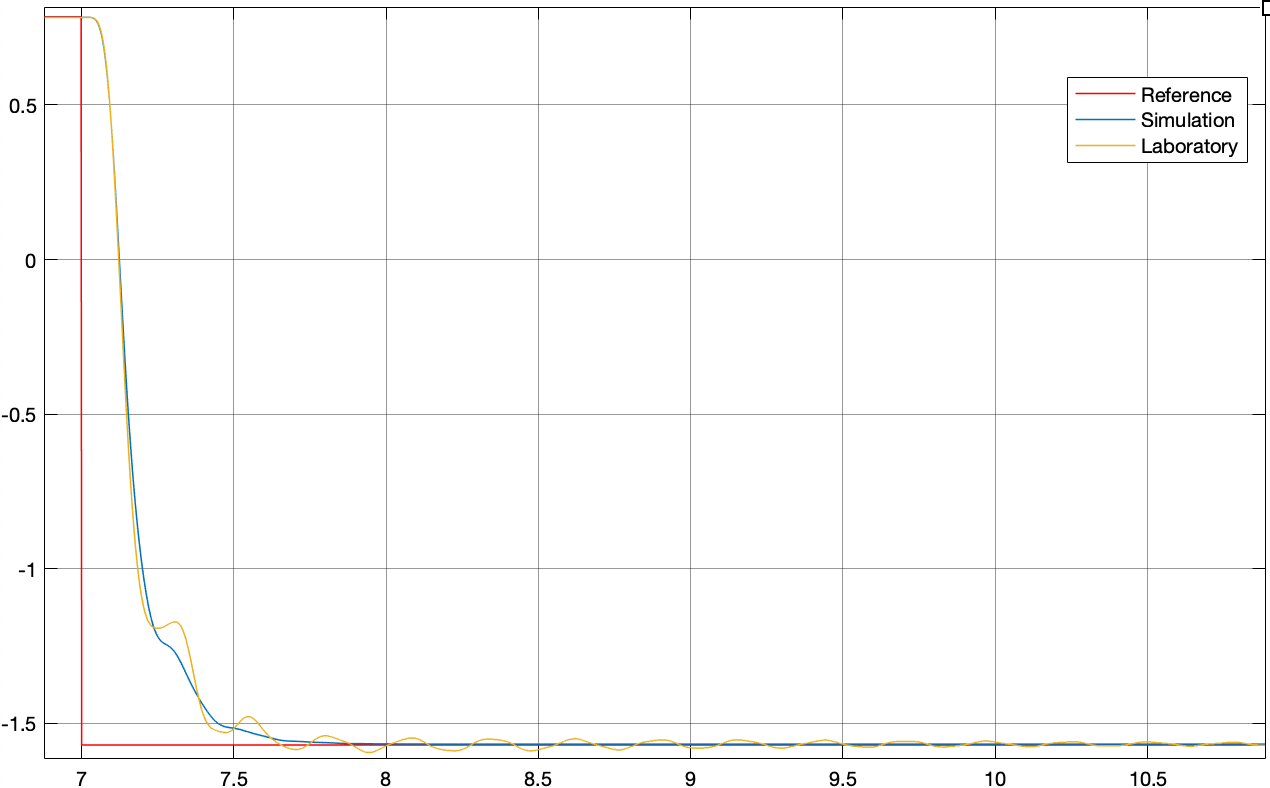
\includegraphics[scale=0.37]{pi_2H}
		\caption{Position step from $\frac{\pi}{4}$ to $-\frac{\pi}{2}$}
	\end{subfigure}
	\\
	\begin{subfigure}{0.5\columnwidth}
		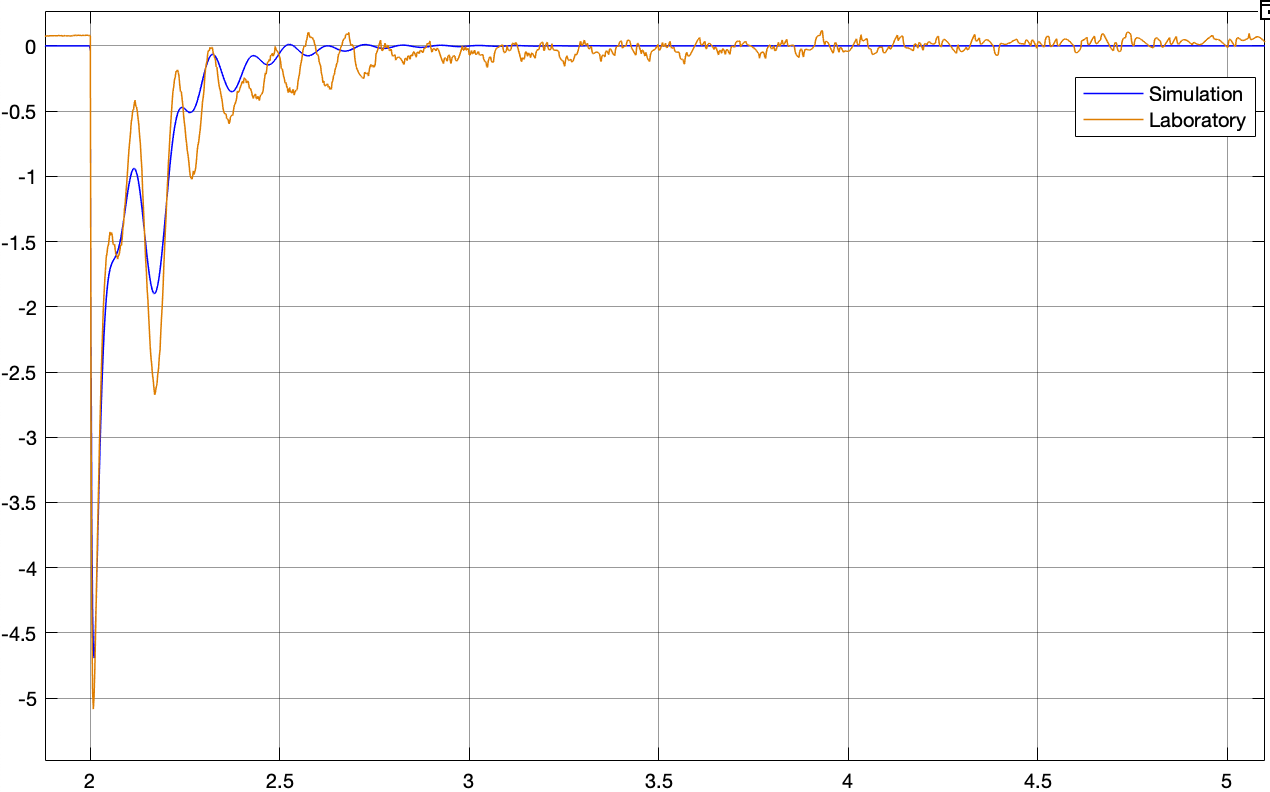
\includegraphics[scale= 0.37]{pi_4Hvolt}
		\caption{Voltage for a step of $\frac{\pi}{4}$}
	\end{subfigure}
	\begin{subfigure}{0.45\columnwidth}
		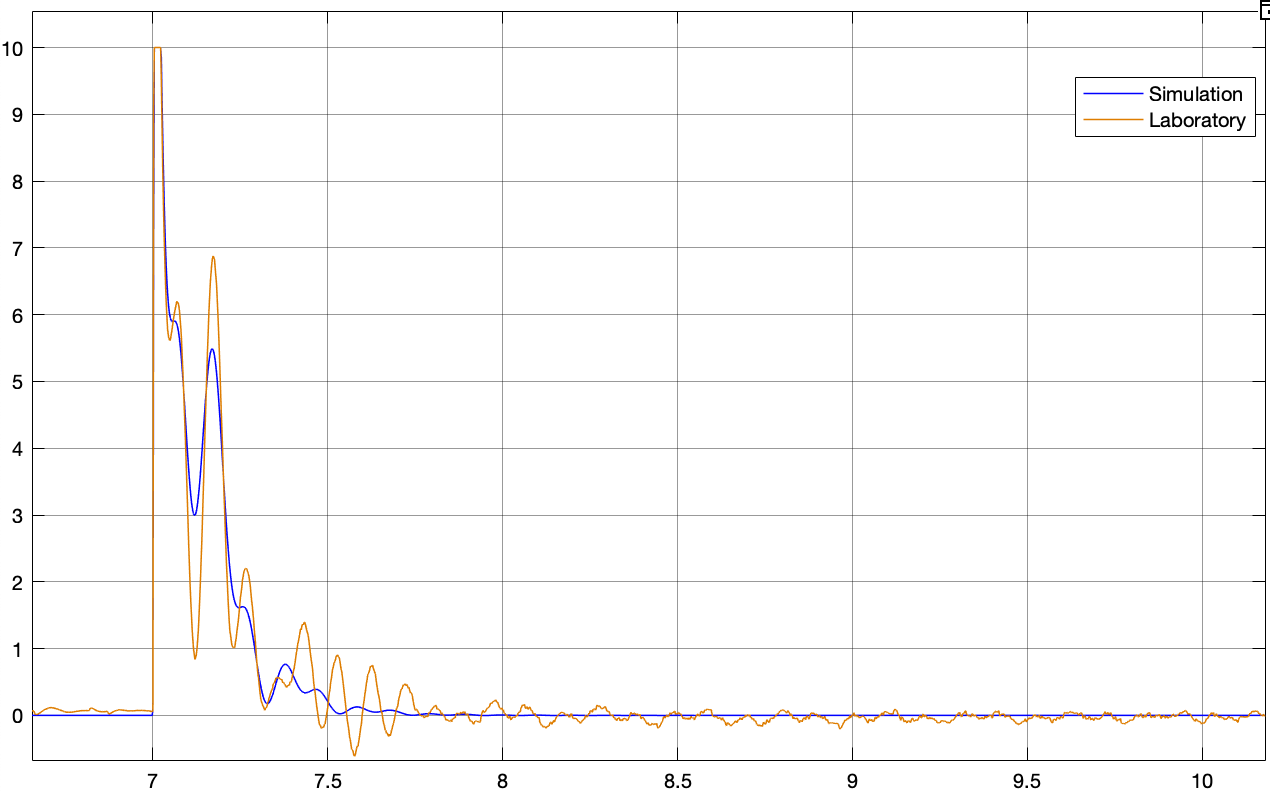
\includegraphics[scale=0.37]{pi_2Hvolt}
		\caption{Voltage for a step from $\frac{\pi}{4}$ to $-\frac{\pi}{2}$}
	\end{subfigure}
	\caption{Position steps response}
	\label{fig:posH2dof}
\end{figure*}




 


